\documentclass[aspectratio=169,11pt]{beamer}

\usetheme{Madrid}
\usecolortheme{seahorse}
\setbeamertemplate{navigation symbols}{}
\setbeamertemplate{footline}{\hfill\scriptsize\insertframenumber/\inserttotalframenumber\hspace{1em}\vspace{0.5em}}

\usepackage[utf8]{inputenc}
\usepackage[T1]{fontenc}
\usepackage{amsmath,amssymb}
\usepackage{graphicx}
\usepackage{booktabs}

\title{Coeficiente de Reflexi\'on de un Panel Ligeramente Conductivo}
\subtitle{M\'etodo FDTD vs Matriz de Transferencia}
\author{M\'etodos Computacionales en F\'isica No Lineal}
\institute{M\'aster en F\'isica y Matem\'aticas --- Universidad de Granada}
\date{Curso 2025--2026}

\begin{document}

% ============================================================
\begin{frame}
\titlepage
\end{frame}

% ============================================================
\begin{frame}{Planteamiento del problema y m\'etodo anal\'itico}

\begin{columns}[T]
\begin{column}{0.55\textwidth}
\textbf{Objetivo:} Calcular $R(f)$ y $T(f)$ de un panel con baja conductividad.

\vspace{0.5em}
\textbf{Dos m\'etodos independientes:}
\begin{enumerate}
  \item Matriz de Transferencia (TMM) --- anal\'itico
  \item FDTD --- num\'erico
\end{enumerate}

\vspace{0.5em}
\textbf{Matriz ABCD} para un panel homog\'eneo de espesor $d$:
\[
\Phi = \begin{pmatrix} \cosh(\gamma d) & \eta\sinh(\gamma d) \\ \sinh(\gamma d)/\eta & \cosh(\gamma d) \end{pmatrix}
\]

donde:
\begin{itemize}
  \item $\varepsilon_c = \varepsilon_r - j\sigma/\omega$ \quad (permitividad compleja)
  \item $\gamma = j\omega\sqrt{\mu_r\varepsilon_c}$ \quad (cte. propagaci\'on)
  \item $\eta = \sqrt{\mu_r/\varepsilon_c}$ \quad (impedancia)
\end{itemize}

\vspace{0.3em}
Coeficientes: \; $R = \frac{A+B-C-D}{A+B+C+D}$, \; $T = \frac{2}{A+B+C+D}$

\vspace{0.3em}
\textbf{Multicapa:} $\Phi_{\text{total}} = \Phi_1 \cdot \Phi_2 \cdots \Phi_N$
\end{column}

\begin{column}{0.42\textwidth}
\centering
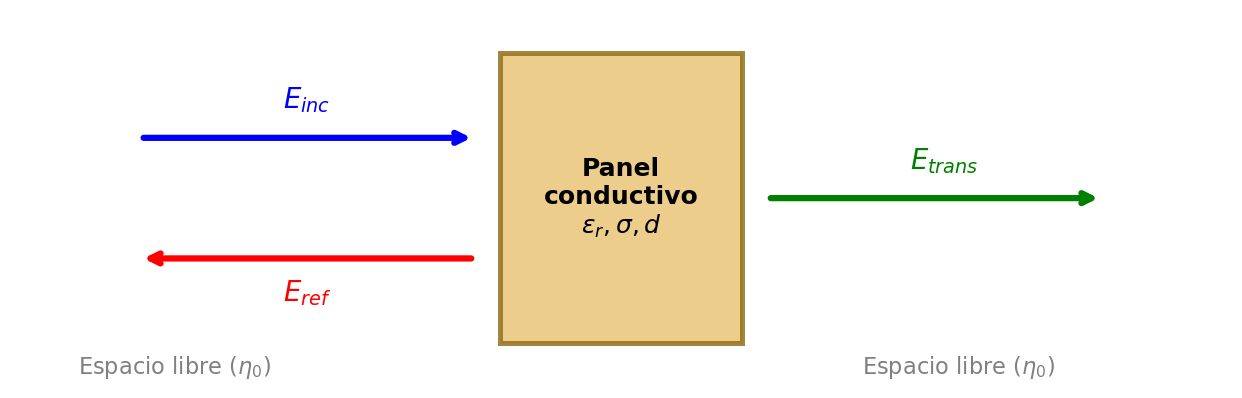
\includegraphics[width=\textwidth]{_figs/esquema.png}

\vspace{0.8em}
{\footnotesize\textbf{Procedimiento FDTD:}
\begin{enumerate}\setlength\itemsep{0pt}
  \item Dominio $[0,L]$ con Mur ABC
  \item Pulso gaussiano $\to$ derecha
  \item Panel en el centro
  \item Observadores izq/der
  \item Referencia sin panel
  \item $R(f), T(f)$ v\'ia FFT
\end{enumerate}}
\end{column}
\end{columns}

\end{frame}

% ============================================================
\begin{frame}{Resultados: FDTD vs Anal\'itico}

\begin{columns}[T]
\begin{column}{0.7\textwidth}
\centering
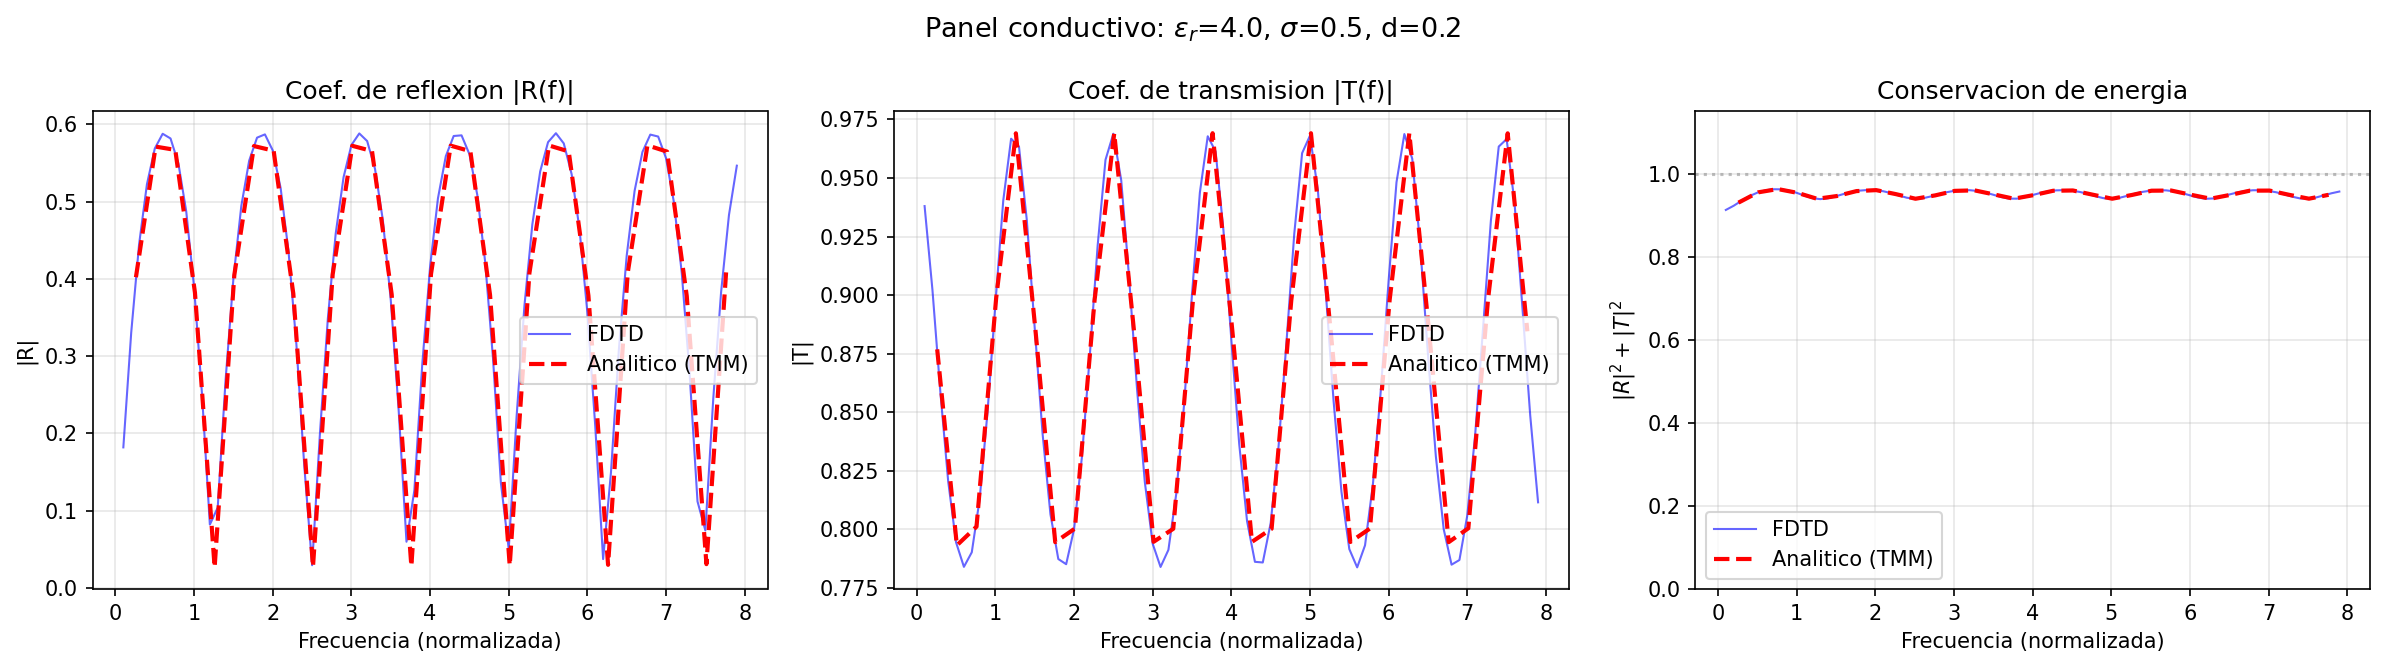
\includegraphics[width=\textwidth]{_figs/comparacion_RT.png}

\vspace{0.3em}
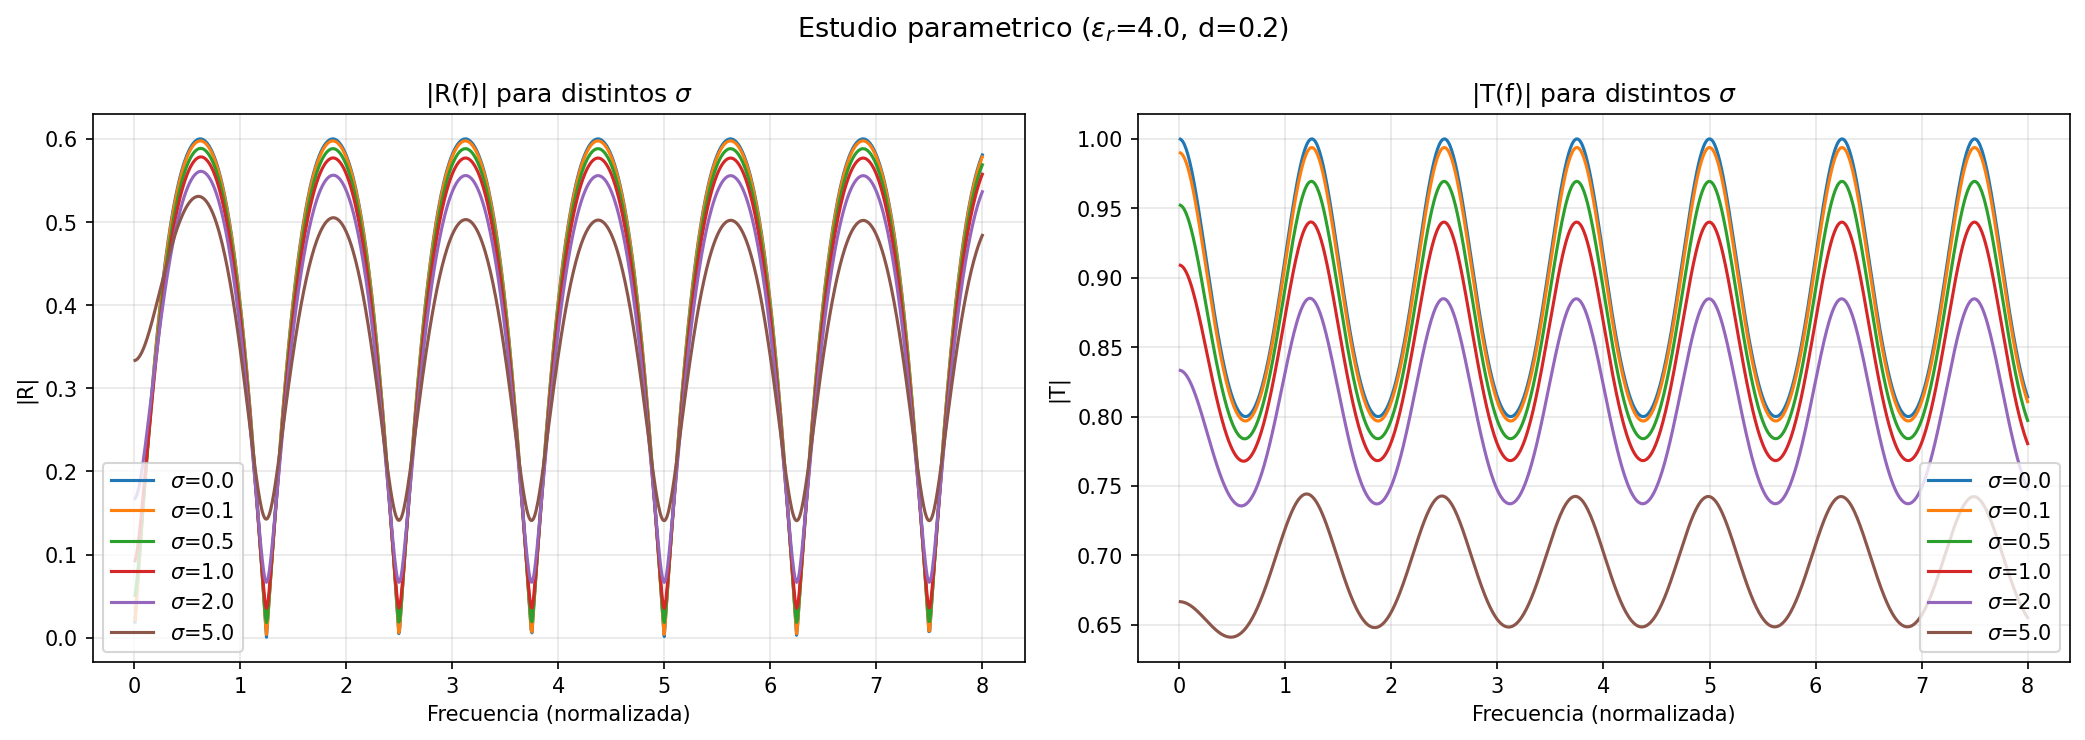
\includegraphics[width=0.48\textwidth]{_figs/barrido_sigma.png}
\hfill
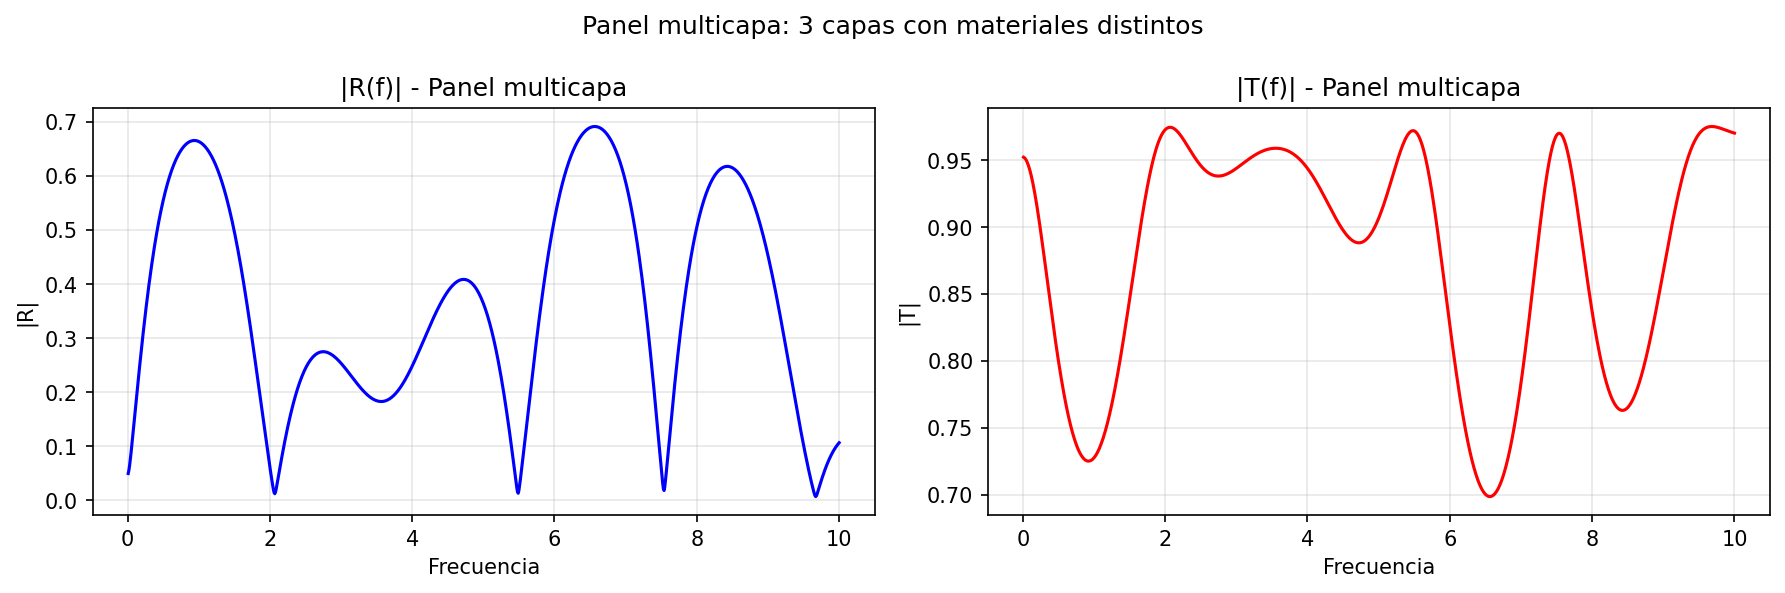
\includegraphics[width=0.48\textwidth]{_figs/multicapa.png}
\end{column}

\begin{column}{0.28\textwidth}
\textbf{Conclusiones:}
\begin{itemize}\setlength\itemsep{0.4em}
  \item Excelente concordancia FDTD vs TMM
  \item $|R|^2 + |T|^2 < 1$ para medios con p\'erdidas (energ\'ia absorbida)
  \item Mayor $\sigma$ $\Rightarrow$ mayor reflexi\'on, menor transmisi\'on
  \item Oscilaciones Fabry--P\'erot se amortiguan con $\sigma$
  \item \textbf{Bonus:} panel multicapa con 3 capas distintas, patr\'on de interferencia m\'as complejo
\end{itemize}
\end{column}
\end{columns}

\end{frame}

% ============================================================
\begin{frame}{Estructura del c\'odigo y validaci\'on}

\begin{columns}[T]
\begin{column}{0.48\textwidth}
\textbf{Arquitectura del repositorio:}

\vspace{0.5em}
\begin{tabular}{@{}ll@{}}
\toprule
\textbf{Archivo} & \textbf{Funci\'on} \\
\midrule
\texttt{fdtd1d.py} & Clase FDTD1D base \\
 & \texttt{set\_panel()} \\
 & \texttt{set\_multilayer()} \\
 & \texttt{run\_panel\_experiment()} \\
\midrule
\texttt{panel\_transfer\_matrix.py} & TMM anal\'itico \\
 & $R(f)$, $T(f)$ exactos \\
\midrule
\texttt{panel\_tests.py} & 10 tests (pytest) \\
\midrule
\texttt{conductive\_panel/} & Visualizaciones \\
 & y comparaciones \\
\bottomrule
\end{tabular}

\vspace{0.5em}
{\small Separaci\'on clara: FDTD num\'erico $\leftrightarrow$ TMM anal\'itico $\leftrightarrow$ tests $\leftrightarrow$ visualizaci\'on.}
\end{column}

\begin{column}{0.50\textwidth}
\textbf{Suite de tests (18 tests, todos pasan):}

\vspace{0.3em}
{\small
\textbf{Tests unitarios:}
\begin{itemize}\setlength\itemsep{0pt}
  \item \texttt{set\_panel} asigna $\varepsilon_r$ y $\sigma$ correctamente
  \item \texttt{set\_multilayer} asigna propiedades por capa
  \item Panel vac\'io: $R=0$, $T=1$
  \item Sin p\'erdidas: $|R|^2+|T|^2=1$
  \item Con p\'erdidas: $|R|^2+|T|^2<1$
  \item Stack 1 capa = panel simple
\end{itemize}

\vspace{0.3em}
\textbf{Tests de integraci\'on:}
\begin{itemize}\setlength\itemsep{0pt}
  \item FDTD panel simple vs TMM (corr $>0.90$)
  \item FDTD multicapa vs TMM (corr $>0.90$)
  \item FDTD espacio libre: $|R| \approx 0$
\end{itemize}
}

\vspace{0.5em}
\centering
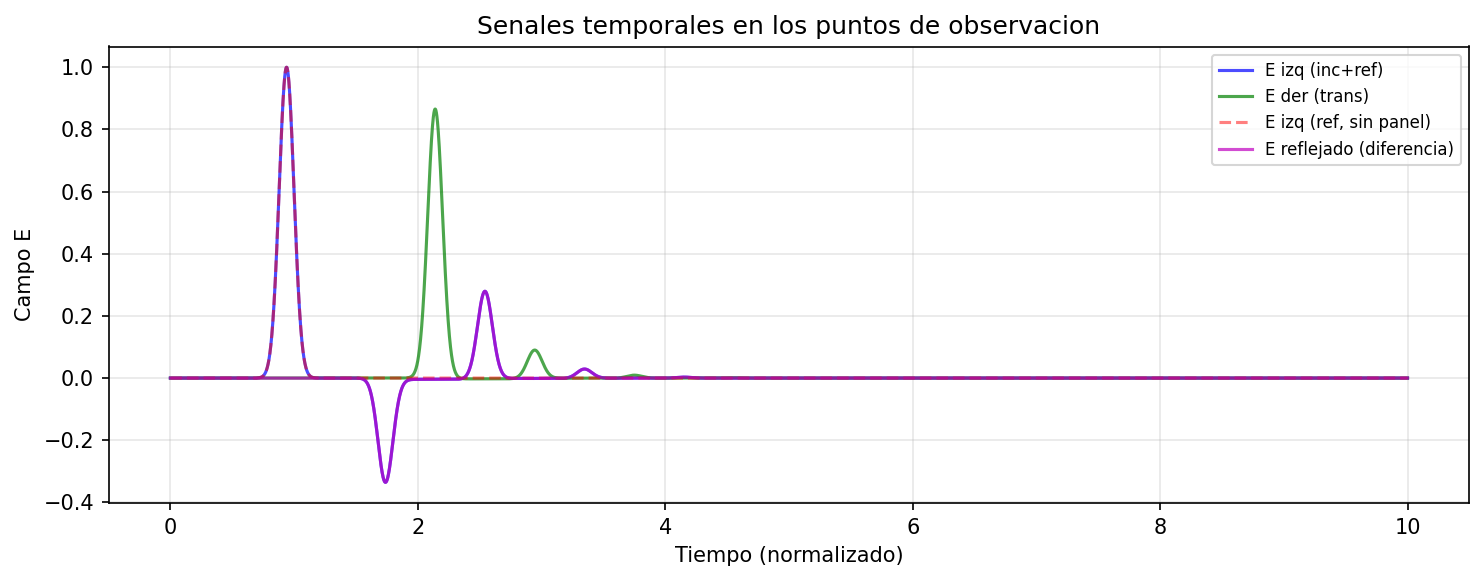
\includegraphics[width=0.85\textwidth]{_figs/temporal.png}
\end{column}
\end{columns}

\end{frame}

\end{document}
